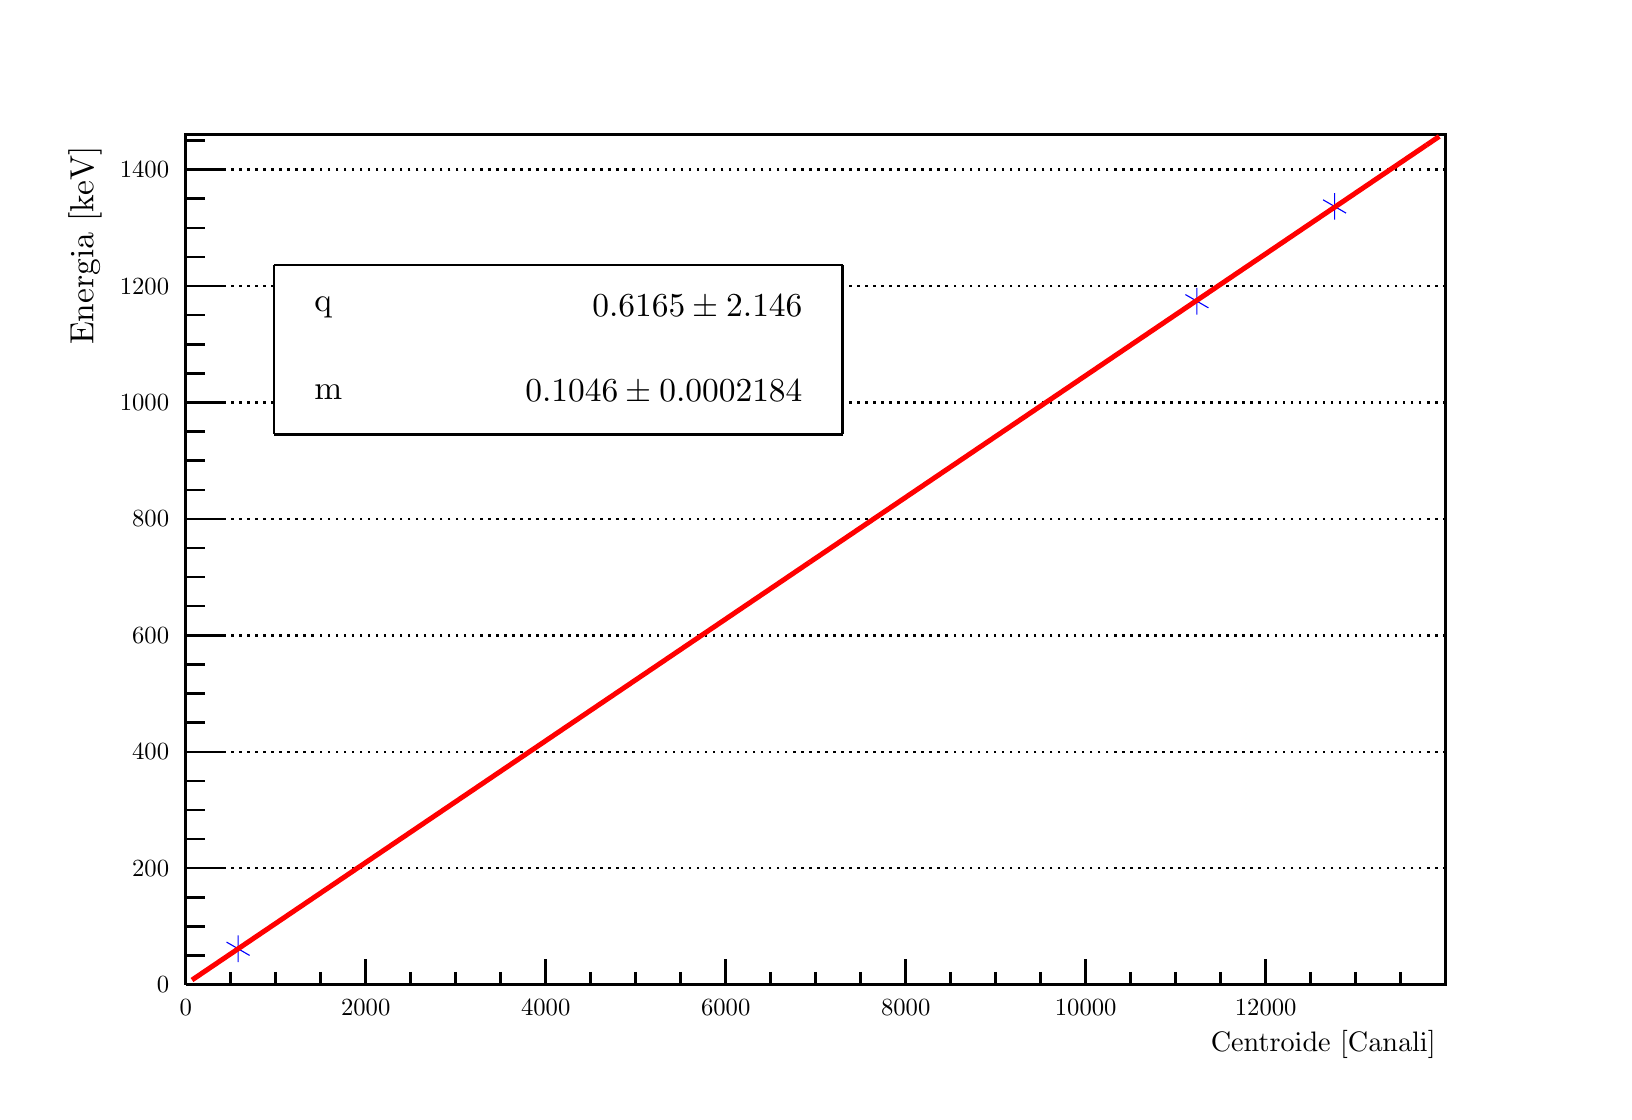
\begin{tikzpicture}
\pgfdeclareplotmark{cross} {
\pgfpathmoveto{\pgfpoint{-0.3\pgfplotmarksize}{\pgfplotmarksize}}
\pgfpathlineto{\pgfpoint{+0.3\pgfplotmarksize}{\pgfplotmarksize}}
\pgfpathlineto{\pgfpoint{+0.3\pgfplotmarksize}{0.3\pgfplotmarksize}}
\pgfpathlineto{\pgfpoint{+1\pgfplotmarksize}{0.3\pgfplotmarksize}}
\pgfpathlineto{\pgfpoint{+1\pgfplotmarksize}{-0.3\pgfplotmarksize}}
\pgfpathlineto{\pgfpoint{+0.3\pgfplotmarksize}{-0.3\pgfplotmarksize}}
\pgfpathlineto{\pgfpoint{+0.3\pgfplotmarksize}{-1.\pgfplotmarksize}}
\pgfpathlineto{\pgfpoint{-0.3\pgfplotmarksize}{-1.\pgfplotmarksize}}
\pgfpathlineto{\pgfpoint{-0.3\pgfplotmarksize}{-0.3\pgfplotmarksize}}
\pgfpathlineto{\pgfpoint{-1.\pgfplotmarksize}{-0.3\pgfplotmarksize}}
\pgfpathlineto{\pgfpoint{-1.\pgfplotmarksize}{0.3\pgfplotmarksize}}
\pgfpathlineto{\pgfpoint{-0.3\pgfplotmarksize}{0.3\pgfplotmarksize}}
\pgfpathclose
\pgfusepathqstroke
}
\pgfdeclareplotmark{cross*} {
\pgfpathmoveto{\pgfpoint{-0.3\pgfplotmarksize}{\pgfplotmarksize}}
\pgfpathlineto{\pgfpoint{+0.3\pgfplotmarksize}{\pgfplotmarksize}}
\pgfpathlineto{\pgfpoint{+0.3\pgfplotmarksize}{0.3\pgfplotmarksize}}
\pgfpathlineto{\pgfpoint{+1\pgfplotmarksize}{0.3\pgfplotmarksize}}
\pgfpathlineto{\pgfpoint{+1\pgfplotmarksize}{-0.3\pgfplotmarksize}}
\pgfpathlineto{\pgfpoint{+0.3\pgfplotmarksize}{-0.3\pgfplotmarksize}}
\pgfpathlineto{\pgfpoint{+0.3\pgfplotmarksize}{-1.\pgfplotmarksize}}
\pgfpathlineto{\pgfpoint{-0.3\pgfplotmarksize}{-1.\pgfplotmarksize}}
\pgfpathlineto{\pgfpoint{-0.3\pgfplotmarksize}{-0.3\pgfplotmarksize}}
\pgfpathlineto{\pgfpoint{-1.\pgfplotmarksize}{-0.3\pgfplotmarksize}}
\pgfpathlineto{\pgfpoint{-1.\pgfplotmarksize}{0.3\pgfplotmarksize}}
\pgfpathlineto{\pgfpoint{-0.3\pgfplotmarksize}{0.3\pgfplotmarksize}}
\pgfpathclose
\pgfusepathqfillstroke
}
\pgfdeclareplotmark{newstar} {
\pgfpathmoveto{\pgfqpoint{0pt}{\pgfplotmarksize}}
\pgfpathlineto{\pgfqpointpolar{44}{0.5\pgfplotmarksize}}
\pgfpathlineto{\pgfqpointpolar{18}{\pgfplotmarksize}}
\pgfpathlineto{\pgfqpointpolar{-20}{0.5\pgfplotmarksize}}
\pgfpathlineto{\pgfqpointpolar{-54}{\pgfplotmarksize}}
\pgfpathlineto{\pgfqpointpolar{-90}{0.5\pgfplotmarksize}}
\pgfpathlineto{\pgfqpointpolar{234}{\pgfplotmarksize}}
\pgfpathlineto{\pgfqpointpolar{198}{0.5\pgfplotmarksize}}
\pgfpathlineto{\pgfqpointpolar{162}{\pgfplotmarksize}}
\pgfpathlineto{\pgfqpointpolar{134}{0.5\pgfplotmarksize}}
\pgfpathclose
\pgfusepathqstroke
}
\pgfdeclareplotmark{newstar*} {
\pgfpathmoveto{\pgfqpoint{0pt}{\pgfplotmarksize}}
\pgfpathlineto{\pgfqpointpolar{44}{0.5\pgfplotmarksize}}
\pgfpathlineto{\pgfqpointpolar{18}{\pgfplotmarksize}}
\pgfpathlineto{\pgfqpointpolar{-20}{0.5\pgfplotmarksize}}
\pgfpathlineto{\pgfqpointpolar{-54}{\pgfplotmarksize}}
\pgfpathlineto{\pgfqpointpolar{-90}{0.5\pgfplotmarksize}}
\pgfpathlineto{\pgfqpointpolar{234}{\pgfplotmarksize}}
\pgfpathlineto{\pgfqpointpolar{198}{0.5\pgfplotmarksize}}
\pgfpathlineto{\pgfqpointpolar{162}{\pgfplotmarksize}}
\pgfpathlineto{\pgfqpointpolar{134}{0.5\pgfplotmarksize}}
\pgfpathclose
\pgfusepathqfillstroke
}
\definecolor{c}{rgb}{1,1,1};
\draw [color=c, fill=c] (0,0) rectangle (20,13.4957);
\draw [color=c, fill=c] (2,1.34957) rectangle (18,12.1461);
\definecolor{c}{rgb}{0,0,0};
\draw [c,line width=0.9] (2,1.34957) -- (2,12.1461) -- (18,12.1461) -- (18,1.34957) -- (2,1.34957);
\definecolor{c}{rgb}{1,1,1};
\draw [color=c, fill=c] (2,1.34957) rectangle (18,12.1461);
\definecolor{c}{rgb}{0,0,0};
\draw [c,line width=0.9] (2,1.34957) -- (2,12.1461) -- (18,12.1461) -- (18,1.34957) -- (2,1.34957);
\draw [c,line width=0.9] (2,1.34957) -- (18,1.34957);
\draw [c,line width=0.9] (2,1.34957) -- (2,12.1461);
\draw [c,dotted,line width=0.9] (18,1.34957) -- (2,1.34957);
\draw [c,dotted,line width=0.9] (18,2.8282) -- (2,2.8282);
\draw [c,dotted,line width=0.9] (18,4.30682) -- (2,4.30682);
\draw [c,dotted,line width=0.9] (18,5.78545) -- (2,5.78545);
\draw [c,dotted,line width=0.9] (18,7.26408) -- (2,7.26408);
\draw [c,dotted,line width=0.9] (18,8.7427) -- (2,8.7427);
\draw [c,dotted,line width=0.9] (18,10.2213) -- (2,10.2213);
\draw [c,dotted,line width=0.9] (18,11.7) -- (2,11.7);
\draw [c,dotted,line width=0.9] (18,11.7) -- (2,11.7);
\draw [c,line width=0.9] (2,1.34957) -- (18,1.34957);
\draw [anchor= east] (18,0.593811) node[scale=1.01821, color=c, rotate=0]{Centroide [Canali]};
\draw [c,line width=0.9] (2,1.67347) -- (2,1.34957);
\draw [c,line width=0.9] (2.57151,1.51152) -- (2.57151,1.34957);
\draw [c,line width=0.9] (3.14302,1.51152) -- (3.14302,1.34957);
\draw [c,line width=0.9] (3.71452,1.51152) -- (3.71452,1.34957);
\draw [c,line width=0.9] (4.28603,1.67347) -- (4.28603,1.34957);
\draw [c,line width=0.9] (4.85754,1.51152) -- (4.85754,1.34957);
\draw [c,line width=0.9] (5.42905,1.51152) -- (5.42905,1.34957);
\draw [c,line width=0.9] (6.00056,1.51152) -- (6.00056,1.34957);
\draw [c,line width=0.9] (6.57207,1.67347) -- (6.57207,1.34957);
\draw [c,line width=0.9] (7.14357,1.51152) -- (7.14357,1.34957);
\draw [c,line width=0.9] (7.71508,1.51152) -- (7.71508,1.34957);
\draw [c,line width=0.9] (8.28659,1.51152) -- (8.28659,1.34957);
\draw [c,line width=0.9] (8.8581,1.67347) -- (8.8581,1.34957);
\draw [c,line width=0.9] (9.42961,1.51152) -- (9.42961,1.34957);
\draw [c,line width=0.9] (10.0011,1.51152) -- (10.0011,1.34957);
\draw [c,line width=0.9] (10.5726,1.51152) -- (10.5726,1.34957);
\draw [c,line width=0.9] (11.1441,1.67347) -- (11.1441,1.34957);
\draw [c,line width=0.9] (11.7156,1.51152) -- (11.7156,1.34957);
\draw [c,line width=0.9] (12.2871,1.51152) -- (12.2871,1.34957);
\draw [c,line width=0.9] (12.8587,1.51152) -- (12.8587,1.34957);
\draw [c,line width=0.9] (13.4302,1.67347) -- (13.4302,1.34957);
\draw [c,line width=0.9] (14.0017,1.51152) -- (14.0017,1.34957);
\draw [c,line width=0.9] (14.5732,1.51152) -- (14.5732,1.34957);
\draw [c,line width=0.9] (15.1447,1.51152) -- (15.1447,1.34957);
\draw [c,line width=0.9] (15.7162,1.67347) -- (15.7162,1.34957);
\draw [c,line width=0.9] (15.7162,1.67347) -- (15.7162,1.34957);
\draw [c,line width=0.9] (16.2877,1.51152) -- (16.2877,1.34957);
\draw [c,line width=0.9] (16.8592,1.51152) -- (16.8592,1.34957);
\draw [c,line width=0.9] (17.4307,1.51152) -- (17.4307,1.34957);
\draw [anchor=base] (2,0.958195) node[scale=0.890934, color=c, rotate=0]{0};
\draw [anchor=base] (4.28603,0.958195) node[scale=0.890934, color=c, rotate=0]{2000};
\draw [anchor=base] (6.57207,0.958195) node[scale=0.890934, color=c, rotate=0]{4000};
\draw [anchor=base] (8.8581,0.958195) node[scale=0.890934, color=c, rotate=0]{6000};
\draw [anchor=base] (11.1441,0.958195) node[scale=0.890934, color=c, rotate=0]{8000};
\draw [anchor=base] (13.4302,0.958195) node[scale=0.890934, color=c, rotate=0]{10000};
\draw [anchor=base] (15.7162,0.958195) node[scale=0.890934, color=c, rotate=0]{12000};
\draw [c,line width=0.9] (2,1.34957) -- (2,12.1461);
\draw [anchor= east] (0.72,12.1461) node[scale=1.20912, color=c, rotate=90]{Energia [keV]};
\draw [c,line width=0.9] (2.48,1.34957) -- (2,1.34957);
\draw [c,line width=0.9] (2.24,1.71923) -- (2,1.71923);
\draw [c,line width=0.9] (2.24,2.08888) -- (2,2.08888);
\draw [c,line width=0.9] (2.24,2.45854) -- (2,2.45854);
\draw [c,line width=0.9] (2.48,2.8282) -- (2,2.8282);
\draw [c,line width=0.9] (2.24,3.19785) -- (2,3.19785);
\draw [c,line width=0.9] (2.24,3.56751) -- (2,3.56751);
\draw [c,line width=0.9] (2.24,3.93717) -- (2,3.93717);
\draw [c,line width=0.9] (2.48,4.30682) -- (2,4.30682);
\draw [c,line width=0.9] (2.24,4.67648) -- (2,4.67648);
\draw [c,line width=0.9] (2.24,5.04614) -- (2,5.04614);
\draw [c,line width=0.9] (2.24,5.41579) -- (2,5.41579);
\draw [c,line width=0.9] (2.48,5.78545) -- (2,5.78545);
\draw [c,line width=0.9] (2.24,6.15511) -- (2,6.15511);
\draw [c,line width=0.9] (2.24,6.52476) -- (2,6.52476);
\draw [c,line width=0.9] (2.24,6.89442) -- (2,6.89442);
\draw [c,line width=0.9] (2.48,7.26408) -- (2,7.26408);
\draw [c,line width=0.9] (2.24,7.63373) -- (2,7.63373);
\draw [c,line width=0.9] (2.24,8.00339) -- (2,8.00339);
\draw [c,line width=0.9] (2.24,8.37305) -- (2,8.37305);
\draw [c,line width=0.9] (2.48,8.7427) -- (2,8.7427);
\draw [c,line width=0.9] (2.24,9.11236) -- (2,9.11236);
\draw [c,line width=0.9] (2.24,9.48202) -- (2,9.48202);
\draw [c,line width=0.9] (2.24,9.85167) -- (2,9.85167);
\draw [c,line width=0.9] (2.48,10.2213) -- (2,10.2213);
\draw [c,line width=0.9] (2.24,10.591) -- (2,10.591);
\draw [c,line width=0.9] (2.24,10.9606) -- (2,10.9606);
\draw [c,line width=0.9] (2.24,11.3303) -- (2,11.3303);
\draw [c,line width=0.9] (2.48,11.7) -- (2,11.7);
\draw [c,line width=0.9] (2.48,11.7) -- (2,11.7);
\draw [c,line width=0.9] (2.24,12.0696) -- (2,12.0696);
\draw [anchor= east] (1.9,1.34957) node[scale=0.890934, color=c, rotate=0]{0};
\draw [anchor= east] (1.9,2.8282) node[scale=0.890934, color=c, rotate=0]{200};
\draw [anchor= east] (1.9,4.30682) node[scale=0.890934, color=c, rotate=0]{400};
\draw [anchor= east] (1.9,5.78545) node[scale=0.890934, color=c, rotate=0]{600};
\draw [anchor= east] (1.9,7.26408) node[scale=0.890934, color=c, rotate=0]{800};
\draw [anchor= east] (1.9,8.7427) node[scale=0.890934, color=c, rotate=0]{1000};
\draw [anchor= east] (1.9,10.2213) node[scale=0.890934, color=c, rotate=0]{1200};
\draw [anchor= east] (1.9,11.7) node[scale=0.890934, color=c, rotate=0]{1400};
\definecolor{c}{rgb}{1,1,1};
\draw [color=c, fill=c] (3.12321,8.33811) rectangle (10.3438,10.4871);
\definecolor{c}{rgb}{0,0,0};
\draw [c,line width=0.9] (3.12321,8.33811) -- (10.3438,8.33811);
\draw [c,line width=0.9] (10.3438,8.33811) -- (10.3438,10.4871);
\draw [c,line width=0.9] (10.3438,10.4871) -- (3.12321,10.4871);
\draw [c,line width=0.9] (3.12321,10.4871) -- (3.12321,8.33811);
\draw [anchor= west] (3.48424,9.94986) node[scale=1.20912, color=c, rotate=0]{q       };
\draw [anchor= east] (9.98281,9.94986) node[scale=1.20912, color=c, rotate=0]{$ 0.6165 \pm 2.146$};
\draw [anchor= west] (3.48424,8.87536) node[scale=1.20912, color=c, rotate=0]{m       };
\draw [anchor= east] (9.98281,8.87536) node[scale=1.20912, color=c, rotate=0]{$ 0.1046 \pm 0.0002184$};
\definecolor{c}{rgb}{0,0,1};
\foreach \P in {(2.66476,1.80516),(14.8424,10.0287),(16.5903,11.2321)}{\draw[mark options={color=c,fill=c},mark size=4.804805pt,mark=asterisk] plot coordinates {\P};}
\definecolor{c}{rgb}{1,0,0};
\draw [c,line width=1.8] (2.08,1.40824) -- (2.24,1.51645) -- (2.4,1.62467) -- (2.56,1.73288) -- (2.72,1.8411) -- (2.88,1.94931) -- (3.04,2.05753) -- (3.2,2.16574) -- (3.36,2.27396) -- (3.52,2.38217) -- (3.68,2.49039) -- (3.84,2.5986) -- (4,2.70682)
 -- (4.16,2.81503) -- (4.32,2.92325) -- (4.48,3.03146) -- (4.64,3.13968) -- (4.8,3.24789) -- (4.96,3.35611) -- (5.12,3.46432) -- (5.28,3.57254) -- (5.44,3.68075) -- (5.6,3.78897) -- (5.76,3.89718) -- (5.92,4.0054) -- (6.08,4.11361) -- (6.24,4.22183)
 -- (6.4,4.33004) -- (6.56,4.43826) -- (6.72,4.54647) -- (6.88,4.65469) -- (7.04,4.7629) -- (7.2,4.87112) -- (7.36,4.97933) -- (7.52,5.08755) -- (7.68,5.19576) -- (7.84,5.30398) -- (8,5.41219) -- (8.16,5.52041) -- (8.32,5.62862) -- (8.48,5.73684) --
 (8.64,5.84505) -- (8.8,5.95327) -- (8.96,6.06148) -- (9.12,6.1697) -- (9.28,6.27791) -- (9.44,6.38613) -- (9.6,6.49434) -- (9.76,6.60256) -- (9.92,6.71077);
\draw [c,line width=1.8] (9.92,6.71077) -- (10.08,6.81899) -- (10.24,6.9272) -- (10.4,7.03542) -- (10.56,7.14363) -- (10.72,7.25185) -- (10.88,7.36006) -- (11.04,7.46828) -- (11.2,7.57649) -- (11.36,7.68471) -- (11.52,7.79292) -- (11.68,7.90114) --
 (11.84,8.00935) -- (12,8.11757) -- (12.16,8.22578) -- (12.32,8.334) -- (12.48,8.44221) -- (12.64,8.55043) -- (12.8,8.65864) -- (12.96,8.76686) -- (13.12,8.87507) -- (13.28,8.98329) -- (13.44,9.0915) -- (13.6,9.19972) -- (13.76,9.30793) --
 (13.92,9.41615) -- (14.08,9.52436) -- (14.24,9.63258) -- (14.4,9.74079) -- (14.56,9.84901) -- (14.72,9.95722) -- (14.88,10.0654) -- (15.04,10.1737) -- (15.2,10.2819) -- (15.36,10.3901) -- (15.52,10.4983) -- (15.68,10.6065) -- (15.84,10.7147) --
 (16,10.8229) -- (16.16,10.9312) -- (16.32,11.0394) -- (16.48,11.1476) -- (16.64,11.2558) -- (16.8,11.364) -- (16.96,11.4722) -- (17.12,11.5804) -- (17.28,11.6887) -- (17.44,11.7969) -- (17.6,11.9051) -- (17.76,12.0133);
\draw [c,line width=1.8] (17.76,12.0133) -- (17.92,12.1215);
\definecolor{c}{rgb}{1,1,1};
\draw [color=c, fill=c] (3.12321,8.33811) rectangle (10.3438,10.4871);
\definecolor{c}{rgb}{0,0,0};
\draw [c,line width=0.9] (3.12321,8.33811) -- (10.3438,8.33811);
\draw [c,line width=0.9] (10.3438,8.33811) -- (10.3438,10.4871);
\draw [c,line width=0.9] (10.3438,10.4871) -- (3.12321,10.4871);
\draw [c,line width=0.9] (3.12321,10.4871) -- (3.12321,8.33811);
\draw [anchor= west] (3.48424,9.94986) node[scale=1.20912, color=c, rotate=0]{q       };
\draw [anchor= east] (9.98281,9.94986) node[scale=1.20912, color=c, rotate=0]{$ 0.6165 \pm 2.146$};
\draw [anchor= west] (3.48424,8.87536) node[scale=1.20912, color=c, rotate=0]{m       };
\draw [anchor= east] (9.98281,8.87536) node[scale=1.20912, color=c, rotate=0]{$ 0.1046 \pm 0.0002184$};
\draw (9.51289,12.8653) node[scale=1.40004, color=c, rotate=0]{};
\end{tikzpicture}
